%!TEX root = ../main.tex

\section{Разностная схема для одномерной задачи}
\label{sec:differential_scheme}

Будем численно решать задачу Коши в области $[0, W]_x \times [0, +\infty)_t$ для уравнения~\eqref{eq:one_dim} и граничных условий
\begin{equation}
    \phi(x, 0) = \phi_0(x); \quad \phi(0, t) = \phi_l(t); \quad \phi(W, t) = \phi_r(t) \tpoint
    \label{eq:cauchy_borders}
\end{equation}

Используем регулярную сетку с временным шагом $\tau$ и пространственным $h$. Пусть $N = W / h$ -- целое число. Пусть $(jh, k \tau)$ -- узлы сетки, $j = \overline{0, N}, \; k \in \Natural_0$. Обозначим $\phi_j^k$ значение сеточной функции $\phi$ в узле $(jh, k \tau)$. Перейдем к следующей разностной задаче:
\begin{equation}
    \cfrac{1}{m} \cfrac{\phi_j^{k + 1} - \phi_j^k}{\tau} = \half K_\phi^2 \epsilon'(\phi_j^k) + \cfrac{\Gamma}{l^2} f'(\phi_j^k) + \cfrac{\Gamma}{2} \cfrac{\phi_{j + 1}^k - 2 \phi_j^k + \phi_{j - 1}^k}{h^2} \tpoint
    \label{eq:subtractive}
\end{equation}
Имеем четырехточечную явную разностную схему:
\begin{numcases}{}
    \mbox{$\begin{aligned}
        \phi_j^{k + 1} = \phi_j^k + m \tau \left( \half K_\Phi^2 \epsilon'(\phi_j^k) + \cfrac{\Gamma}{l^2} f'(\phi_j^k) + \cfrac{\Gamma}{2} \cfrac{\phi_{j + 1}^k - 2 \phi_j^k + \phi_{j - 1}^k}{h^2} \right), \\ j = \overline{1, N - 1}, \quad k \in \Natural_0 \tsemicolon
    \end{aligned}$}
    \label{sch:transition} \\
    \phi_j^0 = \phi_0(jh); \quad \phi_0^k = \phi_l(k \tau); \quad \phi_N^k = \phi_r(k \tau) \tpoint
    \label{sch:borders}
\end{numcases}

Легко видеть, что схема имеет первый порядок аппроксимации по времени и второй порядок аппроксимации по пространственной переменной $x$.

Получим необходимое условие устойчивости по принципу <<замороженных коэффициентов>> (см., например, \cite{bahvalov_computational_methods}). Пусть $\phi_j^k$ и $\phi_j^k + \delta_j^k$ -- решения разностного уравнения~\eqref{eq:subtractive}. Подставим в него $\phi_j^k + \delta_j^k$, получим:
\begin{multline*}
    \cfrac{1}{m} \cfrac{(\phi_j^{k + 1} + \delta_j^{k + 1}) - (\phi_j^k + \delta_j^k)}{\tau} = \half K_\Phi^2 [\epsilon'(\phi_j^k) + \epsilon''(\phi_j^k) \delta_j^k + o(\delta_j^k)] + \\ + \cfrac{\Gamma}{l^2} [f'(\phi_j^k) + f''(\phi_j^k) \delta_j^k + o(\delta_j^k)] + \cfrac{\Gamma}{2} \cfrac{(\phi_{j + 1}^k + \delta_{j + 1}^k) - 2 (\phi_j^k + \delta_j^k) + (\phi_{j - 1}^k + \delta_{j - 1}^k)}{h^2} \tpoint
\end{multline*}
Линеаризуем по возмущению $\delta_j^k$ в точке $\phi_j^k = P$ и сократим слагаемые, учитывая, что $\phi_j^k$ есть решение разностной задачи:
\begin{equation}
    \delta_j^{k + 1} = \delta_j^k + m \tau \left( \half K_\Phi^2 \epsilon''(P) \delta_j^k + \cfrac{\Gamma}{l^2} f''(P) \delta_j^k + \cfrac{\Gamma}{2} \cfrac{\delta_{j + 1}^k - 2 \delta_j^k + \delta_{j - 1}^k}{h^2} \right) \tpoint
    \label{eq:scheme_variation}
\end{equation} 

Применим спектральный признак устойчивости. Пусть $\delta_j^k = \lambda(\theta)^k \exp(\imath j \theta)$, $\imath^2 = -1$; подставим в уравнение \eqref{eq:scheme_variation} выражение для $\delta_j^k$ и, сократив на $\lambda(\theta)^k \exp(\imath j \theta)$, получим:
$$\lambda(\theta) = 1 + m \tau \left( \half K_\Phi^2 \epsilon''(P) + \cfrac{\Gamma}{l^2} f''(P) + \cfrac{\Gamma}{2} \cfrac{e^{\imath \theta} - 2 + e^{-\imath \theta}}{h^2} \right) \tcomma$$
или
\begin{equation}
    \lambda(\theta) = 1 + m \tau \left( \half K_\Phi^2 \epsilon''(P) + \cfrac{\Gamma}{l^2} f''(P) - \cfrac{2 \Gamma}{h^2} \sin^2 \cfrac{\theta}{2} \right) \tpoint
    \label{eq:spectral}
\end{equation}

Согласно спектральному признаку, связь $\tau = \tau(h)$ дает устойчивые вычисления в области $[0, W]_x \times [0, T]_t$ при $\tau, h \to 0$, если существует $C > 0$, такое что для любого~$\theta$ выполнено $|\lambda(\theta)| \leqslant e^{C\tau}$. Заметим, что можно использовать условие $|\lambda(\theta)| \leqslant 1 + C\tau$, как более сильное. Если же для любого $\theta$ выполнено $|\lambda(\theta)| \leqslant 1$, то устойчивыми будут вычисления в области $[0, W]_x \times [0, +\infty)_t$ с бесконечным временным интервалом. Строго говоря, условие спектрального метода необходимое, но не достаточное для устойчивости разностной схемы. Однако на практике устойчивость следует ожидать.

Для начала рассмотрим выражение \eqref{eq:spectral} в точке $P = 0$. Имеем $f''(0) = 0, \; \epsilon''(0) = 0$. Уравнение \eqref{eq:spectral} принимает вид
$$\lambda(\theta) = 1 - \cfrac{2 \tau m \Gamma}{h^2} \sin^2 \cfrac{\theta}{2} \tpoint$$
Значит, для любого $\theta$ выполнено $|\lambda(\theta)| \leqslant 1$, если и только если
\begin{equation}
     \tau \leqslant \cfrac{h^2}{m \Gamma} \tpoint
     \label{cond:spectral_0}
\end{equation}
При выполнении условия \eqref{cond:spectral_0} следует ожидать устойчивый расчет при полностью разрушенной или близкой к таковой среде ($\phi \approx 0$) в области $[0, W]_x \times [0, +\infty)_t$ с бесконечным временным интервалом.

Заметим, что при условии \eqref{cond:spectral_0} к тому же ожидается устойчивый расчет на множестве $[0, W]_x \times [0, T]_t$ при любом $\phi$. В этом случае справедливо неравенство
$$|\lambda(\theta)| \leqslant 1 + m \tau \left| \half K_\Phi^2 \epsilon''(P) + \cfrac{\Gamma}{l^2} f''(P) \right| \tpoint$$
Значит, для некоторого $C$ верно $|\lambda(\theta)| \leqslant 1 + C \tau$, так как $\epsilon''(\phi)$ и $f''(\phi)$ -- непрерывные на отрезке $[0, 1]$ функции. Следует отметить, что, несмотря на подобную универсальность, оценка \eqref{cond:spectral_0} плохо применима на практике и нуждается в уточнении, которое будет сделано позже.

Теперь рассмотрим выражение \eqref{eq:spectral} в точке $P = 1$. Имеем $f''(1) < 0, \; \epsilon''(1) > 0$. Заметим, что при $(K_\Phi^2 / 2) \epsilon''(1) + (\Gamma / l^2) f''(1) \leqslant 0$ можно добиться $|\lambda(\theta)| \leqslant 1$, потребовав, подобно условию \eqref{cond:spectral_0}, $\tau \leqslant h^2 / (2m \Gamma)$ и притом достаточно малое $\tau$. Если подставить в упомянутое неравенство значения $f''(1) = -12, \; \epsilon''(1) = 12 \epsilon_0 / (1 + \delta)^2$ (см. выражение~\eqref{eq:epsilon_phi_phi}), то оно преобразуется в
\begin{equation}
    \cfrac{K_\Phi^2 l^2 \epsilon_0}{2 \Gamma (1 + \delta)^2} \leqslant 1 \tpoint
    \label{cond:spectral_possible_1}
\end{equation}

Итак, при условии \eqref{cond:spectral_possible_1} ожидается существование таких $\tau$ и $h$, что расчет устойчив при $\phi \approx 1$ на множестве с бесконечным временным интервалом. Закономерно, что условие \eqref{cond:spectral_possible_1} эквивалентно условию \eqref{cond:equilibrium_1_stable} устойчивости положения равновесия $\phi \equiv 1$ уравнения \eqref{eq:one_dim}.


\subsection{Улучшенная оценка устойчивости}

В предыдущем разделе из анализа уравнения \eqref{eq:spectral} было получено условие \eqref{cond:spectral_0}, необходимое для устойчивости разностной схемы \eqref{sch:transition}, \eqref{sch:borders} при $\phi \approx 0$. Предположение о его полезности основано на том, что типичным поведением модели будет некоторый процесс перехода $\phi$ от $1$ к $0$ (<<разрушение>>) за конечное время, а затем бесконечно долгое пребывание в состоянии $\phi \approx 0$.

Однако проделанного анализа уравнения \eqref{eq:spectral} в точке $\phi = 0$ недостаточно. В самом деле, было использовано, что $\epsilon''(0) = 0$ (см. выражение \eqref{eq:epsilon_phi_phi}), но не учтено, что $\epsilon''(\phi)$ при малых $\delta$ вблизи $0$ растет очень быстро и достигает больших значений (рис.~\ref{fig:eps_phi_phi}). Получается, что модель, устойчивая в точке $0$, может работать неадекватно в малой ее окрестности. Это нас, конечно, не устраивает -- улучшим оценку устойчивости.

\begin{figure}[!tp]
    \centering
    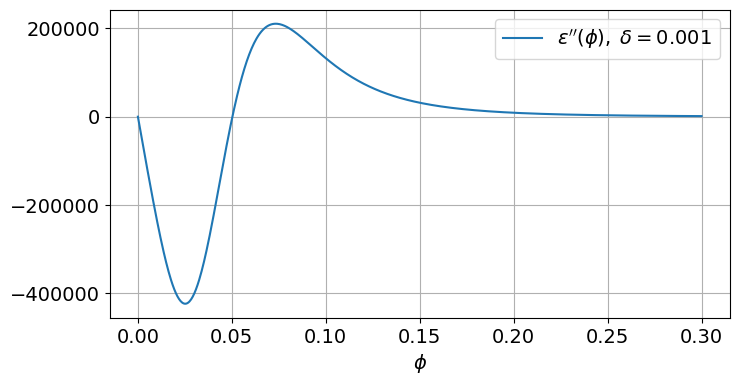
\includegraphics[width=\textwidth]{figures/eps_phi_phi.png}
    \vspace{-0.7cm}
    \caption{Поведение функции $\epsilon''(\phi)$ около $0$.}
    \label{fig:eps_phi_phi}
\end{figure}

Нужно оценить экстремумы функции $\epsilon''(\phi)$ вблизи $0$. Для начала найдем нули $\epsilon'''(\phi)$. Имеем:
$$f'''(\phi) = 24 - 72 \phi; \quad \epsilon'''_{fff} = \cfrac{-6 \epsilon_0}{(f(\phi) + \delta)^4} \tsemicolon$$
\begin{equation}
    \epsilon''' = \epsilon'''_{fff} \cdot (f')^3 + 3 \epsilon''_{ff} \cdot f' \cdot f'' + \epsilon'_f \cdot f''' = \epsilon_0 \cfrac{-6 (f')^3 + 6 (f + \delta) f' f'' - (f + \delta)^2 f'''}{(f + \delta)^4} \tpoint
    \label{eq:epsilon_phi_phi_phi}
\end{equation}
Приравняв $\epsilon'''$ к $0$, получим:
$$-6 (f')^3 + 6 (f + \delta) f' f'' - (f + \delta)^2 f''' = 0 \tcomma$$
или
\begin{multline*}
    -6(12 \phi^2 (1 - \phi))^3 + 6(4 \phi^3 - 3\phi^4 + \delta) \cdot 12 \phi^2 (1 - \phi) \cdot 12 \phi (2 - 3\phi) - \\ - (4 \phi^3 - 3 \phi^4 + \delta)^2 \cdot 24 (1 - 3 \phi) = 0 \tpoint
\end{multline*}
Разделим последнее уравнение на $24\phi^6$, получим:
$$-3 \cdot 12^2 (1 - \phi)^3 + 36 \left(4 - 3\phi + \cfrac{\delta}{\phi^3} \right)(1 - \phi)(2 - 3\phi) - \left(4 - 3 \phi + \cfrac{\delta}{\phi^3} \right)^2 (1 - 3 \phi) = 0 \tpoint$$
Пусть $\delta_n \to +0$ и корень $\phi_n \to +0$, причем $\delta_n / \phi_n^3$ ограничено. Тогда:
$$-3 \cdot 12^2 \cdot 1^3 + 36 \left(4 + \cfrac{\delta_n}{\phi_n^3} \right) \cdot 1 \cdot 2 - \left(4 + \cfrac{\delta_n}{\phi_n^3} \right)^2 \cdot 1 \to 0 \tcomma$$
$$\left(4 + \cfrac{\delta_n}{\phi_n^3} \right)^2 - 72 \left(4 + \cfrac{\delta_n}{\phi_n^3} \right) + 3 \cdot 12^2 \to 0 \tpoint$$
Значит, последовательность $4 + \delta_n / \phi_n^3$ имеет не более двух частичных пределов $\xi_+$ и $\xi_-$ -- корней уравнения $\xi^2 - 72 \xi + 432 = 0$. Первому корню $\xi_+ = 36 + 12 \sqrt{6}$ соответствует
$$\phi = \cfrac{1}{\sqrt[3]{32 + 12 \sqrt{6}}} \sqrt[3]{\delta_n} \approx \cfrac{1}{3.945} \sqrt[3]{\delta_n} \tcomma$$
второму корню $\xi_- = 36 - 12 \sqrt{6}$ соответствует
$$\phi = \cfrac{1}{\sqrt[3]{32 - 12 \sqrt{6}}} \sqrt[3]{\delta_n} \approx \cfrac{1}{1.376} \sqrt[3]{\delta_n} \tpoint$$

Из проделанного рассуждения следует, что при $\delta \to +0$ функция $\epsilon'''(\phi)$ имеет в окрестности $0$ два корня
\begin{equation}
    \phi_{\pm} = \cfrac{1}{\sqrt[3]{32 \pm 12 \sqrt{6}}} \sqrt[3]{\delta} [1 + o(1)] \tpoint
    \label{eq:epsilon_phi_phi_phi_roots}
\end{equation}

Оценим $\epsilon''(\phi)$ в точках $\phi_{\pm}$ при $\delta \to +0$. Пусть $\phi = (1 / c) \sqrt[3]{\delta}, \; c \in \Real$. Тогда:
\begin{multline*}
    \cfrac{\epsilon''}{\epsilon_0} = \cfrac{2(f')^2 - (f + \delta)f''}{(f + \delta)^3} = \cfrac{2 \cdot 12^2 \phi^4 (1 - \phi)^2 - (4 \phi^3 - 3 \phi^4 + \delta) \cdot 12 \phi (2 - 3 \phi)}{(4 \phi^3 - 3 \phi^4 + \delta)^3} = \\ = \cfrac{2 \cdot 12^2 - 8 \cdot 12 - 24 (\delta / \phi^3)}{4^3 + 3 \cdot 4^3 (\delta / \phi^3) + 3 \cdot 4 (\delta / \phi^3)^2 + (\delta / \phi^3)^3} \cdot \cfrac{1}{\phi^5}[1 + o(1)] = c^5 \delta^{-5 / 3} \cfrac{24(8 - c^3)}{(4 + c^3)^3}[1 + o(1)] \tpoint
\end{multline*}
Отсюда:
\begin{equation}
    \epsilon''(\phi_+) \approx -4.378 \epsilon_0 \delta^{-5 / 3}; \quad \epsilon''(\phi_-) \approx 2.216 \epsilon_0 \delta^{-5 / 3} \tpoint
    \label{est:epsilon_phi_phi_bounds}
\end{equation}
Оценки экстремумов $\epsilon''(\phi)$ вблизи $0$ показаны на рис. \ref{fig:eps_phi_phi_multiplied}.

\begin{figure}[!tp]
    \centering
    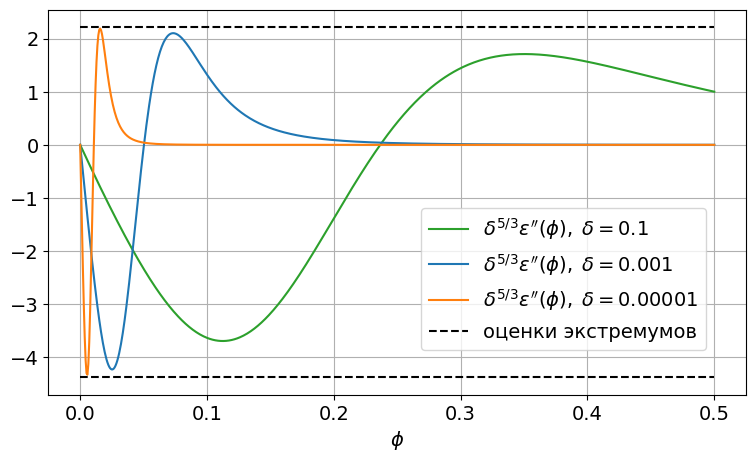
\includegraphics[width=\textwidth]{figures/eps_phi_phi_multiplied.png}
    \caption{Сравнение функций $\delta^{5 / 3} \epsilon''(\phi)$ при различных значениях $\delta$.}
    \label{fig:eps_phi_phi_multiplied}
\end{figure}

Получим новую оценку устойчивости, рассмотрев уравнение \eqref{eq:spectral} в точке $\phi = \phi_+$. $\epsilon''(\phi_+) \approx -4.4 \epsilon_0 \delta^{-5 / 3}$. Сумма в скобках отрицательна ($\delta$ мало, $\epsilon''(\phi_+)$ велико по модулю и отрицательно), поэтому $f''(\phi_0) > 0$ можно считать равным $0$: оценку это только усилит. Преобразовав уравнение \eqref{eq:spectral}, получим:
$$\lambda(\theta) = 1 + m \tau \left( -\cfrac{2.2 K_\Phi^2 \epsilon_0}{\delta^{5 / 3}} - \cfrac{2 \Gamma}{h^2} \sin^2 \cfrac{\theta}{2} \right) \tpoint$$
Условие $|\lambda(\theta)| \leqslant 1$ справедливо для любого $\theta$, если и только если
\begin{equation}
    \tau \leqslant \left( \cfrac{1.1 m K_\Phi^2 \epsilon_0}{\delta^{5 / 3}} + \cfrac{m \Gamma}{h^2} \right)^{-1} \tpoint
    \label{cond:spectral_better_theoretical}
\end{equation}

Для применения на практике оценку \eqref{cond:spectral_better_theoretical} нужно брать <<с запасом>> (экспериментальное обоснование будет дано позже). Сделаем оценку строже, примерно удвоив знаменатель:
\begin{equation}
    \tau \leqslant \cfrac{1}{2m} \left( \cfrac{K_\Phi^2 \epsilon_0}{\delta^{5 / 3}} + \cfrac{\Gamma}{h^2} \right)^{-1} \tpoint
    \label{cond:spectral_better}
\end{equation}

Более простая оценка не слабее оценки \eqref{cond:spectral_better} выглядит следующим образом:
\begin{equation}
    \tau \leqslant \cfrac{1}{4m} \min \left(\cfrac{\delta^{5 / 3}}{K_\Phi^2 \epsilon_0}, \; \cfrac{h^2}{\Gamma} \right) \tpoint
    \label{cond:spectral_better_simpler}
\end{equation}

Полученная оценка \eqref{cond:spectral_better} устойчивости разностной схемы \eqref{sch:transition}, \eqref{sch:borders} содержит все параметры уравнения \eqref{eq:one_dim}, кроме $l$.


\subsection{О сходимости решения разностной задачи}

Если разностная схема аппроксимирует задачу Коши и к тому же обладает устойчивостью при заданной связи $\tau = \tau(h)$, то решение разностной задачи сходится к решению задачи Коши при $h \to 0$. Расшифруем перечисленные понятия более формально.

Далее кратко изложены базовые элементы теории сходимости разностных схем, приближающих линейные дифференциальные задачи. За основу взят материал из книги \cite{bahvalov_computational_methods}; более подробно тема освещена в книге \cite{kalitkin_computational_methods}. Соответствующие определения и утверждения можно сформулировать и для нелинейных задач \cite{kalitkin_computational_methods}, однако для исследуемого уравнения \eqref{eq:one_dim} результативнее будет в ходе нестрогого анализа применить линейную теорию, а затем подтвердить результаты моделированием.

Пусть $\Omega \subset \Real^s$ -- пространство независимых переменных, $\Gamma = \partial \Omega$ -- граница $\Omega$, $\Int \Omega = \Omega \smallsetminus \partial \Omega$ -- внутренность $\Omega$; задан класс $Y$ функций $y(\vx)$ на $\Omega$ (обладающих некоторыми содержательными свойствами, например, гладкостью).

Задан линейный оператор $L: Y \longrightarrow I$, где $I$ -- некоторое пространство функций на $\Int \Omega$; задан линейный оператор $l: Y \longrightarrow G$, где $G$ -- некоторое пространство функций на $\partial \Omega$. Подразумевается, что $L$ и $l$ включают в себя операции дифференцирования. Сформулируем дифференциальную задачу:
\begin{equation}
    \{ \quad Ly = f; \quad ly = g \quad \} \tcomma
    \label{eq:formal_differential}
\end{equation}
где $y(\vx) \in Y$ -- искомая функция, $f \in I, \; g \in G$. Первое уравнение имеет смысл условия на $y$ во внутренности $\Omega$, второе -- краевого условия.

В пространстве $\Omega$ введем сетку, то есть определим некоторое конечное подмножество $\Omega_h \subset \Omega$. Здесь $h$ -- параметр, имеющий смысл мелкости шага сетки, -- то есть, строго говоря, определено семейство сеток. Функцию $y \in Y$ можно ограничить на $\Omega_h$ -- введем обозначение $[y]_h = y|_{\Omega_h}$. Пусть $Y_h = \{[y]_h: y \in Y\}, \; I_h = \{[f]_h: f \in I\}, \; G_h = \{[g]_h: g \in G\}$. Некоторые $L_h: Y_h \longrightarrow I_h$ и $l_h: Y_h \longrightarrow G_h$ будем называть разностными операторами; пусть $L$ и $l$ линейные. Теперь можно сформулировать разностную задачу (строго говоря, семейство задач):
\begin{equation}
    \{ \quad L_h y_h = f_h; \quad l_h y_h = g_h \quad \} \tpoint
    \label{eq:formal_subtractive}
\end{equation}
$y_h \in Y_h$ -- искомая сеточная функция, $f_h \in I_h, \; g_h \in G_h$.

Пусть на пространствах $Y$, $I$, $G$ определены некоторые нормы $\enorm_Y$, $\enorm_I$, $\enorm_G$ соответственно. Пусть на пространстве $Y_h$ определена норма $\enorm_{Y_h}$, такая что $\forall y \in Y \; \norm{[y]_h}_{Y_h} \to \norm{y}_Y$ при $h \to 0$. В этом случае нормы $\enorm_Y$ и $\enorm_{Y_h}$ назовем \emph{согласованными}. Пусть аналогично $\enorm_{I_h}$ и $\enorm_{G_h}$ -- нормы на $I_h$ и $G_h$, согласованные с $\enorm_I$ и $\enorm_G$ соответственно.

Теперь можно формально определить аппроксимацию, устойчивость и сходимость.

Разностная задача \eqref{eq:formal_subtractive} \emph{аппроксимирует} дифференциальную задачу \eqref{eq:formal_differential}, если
\begin{multline*}
\forall y \in Y \quad \norm{[Ly]_h - L_h [y]_h}_{I_h} + \norm{[f]_h - f_h}_{I_h} + \\ + \norm{[ly]_h - l_h [y]_h}_{G_h} + \norm{[g]_h - g_h} = \bigO (h^k) \text{ при } h \to 0 \tpoint
\end{multline*}
Порядок $k$ стремления выражения к $0$ называют порядком аппроксимации.

Решение $y_h$ разностной задачи \eqref{eq:formal_subtractive} \emph{сходится} к решению $y$ дифференциальной задачи \eqref{eq:formal_differential}, если
$$\norm{[y]_h - y_h}_{Y_h} = \bigO (h^k) \text{ при } h \to 0 \tpoint$$
Порядок $k$ стремления выражения к $0$ называют порядком сходимости.

Разностная задача \eqref{eq:formal_subtractive} \emph{устойчива}, если
$$\exists M \in \Real \; \forall h \; \forall z_h \in Y_h \quad \norm{z_h}_{Y_h} \leqslant M \cdot (\norm{L_h z_h}_{I_h} + \norm{l_h z_h}_{G_h}) \tpoint$$

Далее в несколько упрощенном виде, достаточном для дальнейшего исследования, приведем центральное утверждение рассматриваемой теории.

\begin{theorem}[Филиппова]
    Пусть разностная задача \eqref{eq:formal_subtractive} аппроксимирует дифференциальную задачу \eqref{eq:formal_differential}, а также разностная задача устойчива. Тогда решение $y_h$ разностной задачи сходится к решению $y$ дифференциальной задачи, причем с порядком не меньше, чем порядок аппроксимации.
\end{theorem}

[О применении к исследуемой задаче]